\documentclass[]{article}
\usepackage{lmodern}
\usepackage{amssymb,amsmath}
\usepackage{ifxetex,ifluatex}
\usepackage{fixltx2e} % provides \textsubscript
\ifnum 0\ifxetex 1\fi\ifluatex 1\fi=0 % if pdftex
  \usepackage[T1]{fontenc}
  \usepackage[utf8]{inputenc}
\else % if luatex or xelatex
  \ifxetex
    \usepackage{mathspec}
  \else
    \usepackage{fontspec}
  \fi
  \defaultfontfeatures{Ligatures=TeX,Scale=MatchLowercase}
\fi
% use upquote if available, for straight quotes in verbatim environments
\IfFileExists{upquote.sty}{\usepackage{upquote}}{}
% use microtype if available
\IfFileExists{microtype.sty}{%
\usepackage{microtype}
\UseMicrotypeSet[protrusion]{basicmath} % disable protrusion for tt fonts
}{}
\usepackage[margin=1in]{geometry}
\usepackage{hyperref}
\hypersetup{unicode=true,
            pdftitle={Towards the construction of a causal map of the human phenome},
            pdfborder={0 0 0},
            breaklinks=true}
\urlstyle{same}  % don't use monospace font for urls
\usepackage{graphicx,grffile}
\makeatletter
\def\maxwidth{\ifdim\Gin@nat@width>\linewidth\linewidth\else\Gin@nat@width\fi}
\def\maxheight{\ifdim\Gin@nat@height>\textheight\textheight\else\Gin@nat@height\fi}
\makeatother
% Scale images if necessary, so that they will not overflow the page
% margins by default, and it is still possible to overwrite the defaults
% using explicit options in \includegraphics[width, height, ...]{}
\setkeys{Gin}{width=\maxwidth,height=\maxheight,keepaspectratio}
\IfFileExists{parskip.sty}{%
\usepackage{parskip}
}{% else
\setlength{\parindent}{0pt}
\setlength{\parskip}{6pt plus 2pt minus 1pt}
}
\setlength{\emergencystretch}{3em}  % prevent overfull lines
\providecommand{\tightlist}{%
  \setlength{\itemsep}{0pt}\setlength{\parskip}{0pt}}
\setcounter{secnumdepth}{0}
% Redefines (sub)paragraphs to behave more like sections
\ifx\paragraph\undefined\else
\let\oldparagraph\paragraph
\renewcommand{\paragraph}[1]{\oldparagraph{#1}\mbox{}}
\fi
\ifx\subparagraph\undefined\else
\let\oldsubparagraph\subparagraph
\renewcommand{\subparagraph}[1]{\oldsubparagraph{#1}\mbox{}}
\fi
\usepackage{amsmath}

%%% Use protect on footnotes to avoid problems with footnotes in titles
\let\rmarkdownfootnote\footnote%
\def\footnote{\protect\rmarkdownfootnote}

%%% Change title format to be more compact
\usepackage{titling}

% Create subtitle command for use in maketitle
\newcommand{\subtitle}[1]{
  \posttitle{
    \begin{center}\large#1\end{center}
    }
}

\setlength{\droptitle}{-2em}
  \title{Towards the construction of a causal map of the human phenome}
  \pretitle{\vspace{\droptitle}\centering\huge}
  \posttitle{\par}
  \author{}
  \preauthor{}\postauthor{}
  \predate{\centering\large\emph}
  \postdate{\par}
  \date{27 June 2017}

\begin{document}
\maketitle

\subsection{Introduction}\label{introduction}

Mendelian randomisation (MR) (1,2) exploits genetic pleiotropy to infer
the causal relationships between phenotypes. Suppose that one trait (the
exposure) causally influences another (the outcome). If a SNP influences
the outcome through the exposure then the SNP is exhibiting vertical
pleiotropy. Such a genetic variant is considered to be an instrumental
variable for the exposure, and can be exploited to mimic a randomised
controlled trial, enabling a causal estimate to be made by comparing the
outcome phenotypes between those individuals that have the
exposure-increasing allele against those who do not. Multiple
independent genetic variants for a particular exposure can be used
jointly to improve causal inference, because a) each variant is an
independent natural experiment, and an overall causal estimate can be
obtained by meta-analysing the single estimates from each instrument;
and b) some violations of the assumptions of MR (most notably that the
SNP influences the outcome through no pathways other than the exposure)
can be evaluated through sensitivity analyses.

Genome-wide association studies (GWAS) have identified genetic
instrumental variables for thousands of phenotypes. Recent developments
in Mendelian randomisation have enabled knowledge of instrumental
variables to be applied using only summary level data (known as
two-sample MR, 2SMR). Here, in order to infer the causal effect of an
exposure on an outcome all that is required is an estimate of the
genetic effects of the instrumenting SNP on the exposure, and the
corresponding estimate of the effect on the outcome. This has two major
advantages. First, GWAS summary data is non-disclosive and often
publicly available. Second, causal inference can be made between
phenotypes even if they have not been measured in the same samples,
limiting the breadth of possible causal estimates only to the
availability of GWAS summary data for the traits in question.

Problems with obtaining unbiased causal effects can arise, however, if
the genetic instruments exhibit horizontal pleiotropy (HP), where they
influence the outcome through a pathway other than the exposure. The
extent of this problem is not to be understated, and many methods have
been developed that attempt to reliably obtain unbiased causal estimates
under specific models of HP. It is considered best practice to report
estimates from all available methods as sensitivity analyses when
presenting causal estimates, however this strategy is not necessarily
optimal for several reasons. First, if different methods disagree it is
not possible to know which is correct because the appropriate model of
HP is not known. Second, though the IVW approach is most statistically
powerful under no HP, it can have high false negative or low true
positive rates in the presence of HP compared to other methods. Given
that pleiotropy has been hypothesised to be universal, defaulting to the
IVW method in the first instance and using other methods as sensitivity
analyses may not be appropriate. Third, the available methods do not
cover all possible models of HP, and therefore an automated method for
instrument selection may be necessary. Fourth, it could be of interest
to make causal effect estimates for thousands of traits, in which case a
discerning evaluation of each causal effect of interest may not be
possible or convenient.

In this paper we introduce two innovations towards improving the
reliability of MR estimates. First, we introduce an approach to
automatically discard genetic variants that are likely to be invalid.
Second, we hypothesised that characteristics of the summary data could
indicate which method would be most reliable, and we introduce new
machine learning approaches that attempt to automate both instrument and
method selection. Using curated GWAS summary data for thousands of
phenotypes, we use these new methods to construct a graph of millions of
causal estimates. We consider this to be only a `first draft' of the
causal map of the human phenome.

\subsection{Methods}\label{methods}

\subsubsection{GWAS summary data and their use in
2SMR}\label{gwas-summary-data-and-their-use-in-2smr}

The use of summary data in two-sample MR is described in detail
elsewhere. A brief outline of the procedure is as follows. First,
genetic instruments for the exposure trait need to be identified - those
SNPs with \(p < 10^{-8}\) are retained, collecting their effect sizes
and standard errors and effect alleles for the association with the
exposure trait. These can be obtanied manually from complete summary
data or from curated lists of significant GWAS associations. Next, the
effects of those SNPs on the outcome need to be obtained, typically
necessitating complete summary data because it is unlikely that these
SNPs will have reached genome-wide significance (and therefore be
present in curated catalogues). At its most simple implementation, the
regression of the SNP-exposure effect sizes against the SNP-outcome
effect sizes, with greater weight afforded to those SNPs with smaller
SNP-outcome standard errors, provides the estimate of the causal effect
of the exposure on the outcome.

Given summary data for a large number of traits, it is straightforward
to exhaustively analyse the causal relationships of every trait against
every other trait for which there is sufficient summary data available.
Supplementary table X provides a list of all traits that have available
GWAS summary data, indicating if they have complete summary data (in
which case they can be used as both exposure traits and outcome traits),
or if they only have significant associations (in which they can only be
used as exposure traits). Supplementary table X provides a list of the
genetic instruments used for each trait.

\subsubsection{Mendelian randomisation methods and their
assumptions}\label{mendelian-randomisation-methods-and-their-assumptions}

In this paper we consider three main classes of MR estimation. Full
details for each approach have been described extensively elsewhere.

\textbf{Mean-based methods:} Here we consider four nested models. The
inverse variance weighted (IVW) fixed effects meta-analysis approach
assumes that variants exhibit no HP. IVW random effects meta-analysis
relaxes the HP assumption, allowing it to be present but balanced - such
that it only leads to increased heterogeneity around the regression and
not introducing bias. Fixed effects Egger regression relaxes the HP
assumption further by allowing a non-zero intercept which essentially
allows horizontal pleiotropy be directional, where it systematically
occurs in a specific direction. Random effects Egger regression allows
heterogeneity around the directional HP, as long as the HP effects are
not correlated with the SNP-exposure effects (this is the INSIDE
assumption).

The Rucker framework uses estimates of heterogeneity in the IVW and
Egger frameworks to navigate between these nested models. A jackknife
approach (random selection with replacement of instruments) can be used
to obtain a sampling distribution for the model estimate amongst these
four variations. Using 1000 rounds of jackknife estimates, we can obtain
a final estimate using the mean or the median of the distribution. We
only use the jackknife approach for associations where there are 15 or
more variants to avoid combinatorial saturation.

\textbf{Median-based methods:} An alternative approach is to take the
median effect of all available instruments. This has the advantage that
up to half the instruments can be invalid, and the estimate will remain
unbiased. Developing the approach further to allow stronger instruments
to contribute more towards the estimate can be obtained by obtaining the
median of the weights of each instrument. The penalised weighted median
estimator \ldots{}

\textbf{Mode-based methods:} Similar to the median, the mode based
estimator clusters the instruments into groups based on similarity of
causal effects, and returns the final causal effect estimate based on
the cluster that has the largest number of instruments. This can be
extended in two ways, first by weighting the strength of each cluster by
the inverse of the variance of the SNP-outcome associations in the
cluster; second by weighting the strength of each cluster by the inverse
of the variance of the SNP-exposure associations.

\subsubsection{Instrument selection}\label{instrument-selection}

\paragraph{Top hits}\label{top-hits}

The simplest approach to selecting instruments for performing MR is to
take take SNPs that have been declared significant in the published GWAS
for the exposure. This typically involves obtaining SNPs that surpass
\(p < 5 \times 10^{-8}\), using clumping to obtain independent SNPs, and
then replicating in an independent sample. These results are often
recorded in public GWAS catalogs. Alternatively the clumping procedure
can be performed using complete summary data in MR-Base. We call this
the ``top hits'' strategy.

\paragraph{Steiger filtering}\label{steiger-filtering}

With genome-wide association studies growing ever larger, the
statistical power to detect significant associations that may be
influencing the trait downstream of many other pathways increases. For
example, if a SNP \(g_{A}\) influences trait \(A\), and trait \(A\)
influences trait \(B\), then a sufficiently powered GWAS will identify
the \(g_{A}\) as being significant for trait \(B\) (Figure 1a). Using
\(g_{A}\) as an instrument to test the causal effect of \(A\) on \(B\)
is perfectly valid. But in the (incorrectly hypothesised) MR analysis of
trait \(B\) on trait \(A\) could erroneously result in the apparent
causal association of \(B\) on \(A\). If \(g_{A}\) is only one of many
known instruments for \(B\), amongst which some are valid, it is to the
advantage of the researcher to exclude \(g_{A}\) from the analysis.

An approach to inferring the causal direction between phenotypes was
developed recently, using the following basic premise. If trait \(A\)
causes trait \(B\) then

\[
\sum^M_{i=1}{cor(g_{i}, A)^2} > \sum^M_{i=1}{cor(g_{i}, B)^2}
\]

because the \(cor(g_{i}, B)^2 = cor(A, B)^{2} cor(g_{i}, A)^{2}\). This
simple inequality will not hold in some cases, for example
\(\rho_{x, x_o} < \rho_{x,y}\rho_{y,y_o}\) where \(\rho_{x, x_o}\) and
\(\rho_{y, y_o}\) are the precision of the measurements of the \(x\) and
\(y\). Steiger's Z-test of correlated correlations can be used to
formally test the extent to which the two correlations are statistically
different.

Here we adapt this approach to automatically filter SNPs that are liable
to be invalid (Figure 1a). In this case the Steiger test applied to each
variant in turn will identify \(g_{A}\) as being unlikely to primarily
associate with \(B\) relative to \(A\). Similarly, for SNPs that
influence confounders of \(A\) and \(B\) or those variants that exhibit
horizontal pleiotropy, the difference in \(cor(g_{i}, A)^2\) and
\(cor(g_{i}, B)^2\) will be reduced, increasing the likelihood of the
SNP being excluded because the Steiger Z-test is less likely to be
significant.

To estimate \(cor(g, x)^2\), if \(x\) is continuous we obtain the
F-statistic from the reported p-value and sample size and then
\(cor(g, x)^2 = \frac{F}{N - 2 - F}\). If \(x\) is binary then our
objective is to estimate the variance of the risk liability explained by
the SNP, \(cor(g, x)^2 = \frac{V_a}{V_a + V_e}\). Here,
\(V_e = \pi^2/3\), and \(V_a = 2\beta^2p(1-p)\), where \(\beta\) is the
log odds ratio and \(p\) is the allele frequency of the SNP in the
population. \(p\) can be estimated using the allele frequency of the SNP
in an ascertained sample by deriving the \(2 \times 2\) contingency
table from the odds ratio \(e^\beta\), allele frequency in the
ascertained sample \$p\_\{cc\}, and number of cases \(N_1\) and controls
\(N_0\).

\subsubsection{Competitive mixture of
experts}\label{competitive-mixture-of-experts}

We consider 14 MR methods, for which instruments can be supplied using
two instrument selection strategies, leading to 28 methods in total. In
the context of this analysis, each method is considered to be an
`expert', taking a set of SNP-exposure and SNP-outcome effect sizes and
their standard errors as inputs. Our objective is to select the expert
most likely to be correct for a specific MR analysis.

\paragraph{Mixture of experts}\label{mixture-of-experts}

The mixture of experts (MoE) method is a machine learning approach which
seeks to divide a parameter space into subdomains, such that a
particular expert is used primarily for problems that reside in a
subdomain most suited to that expert. In this case our objective is to
identify characteristics of the SNP-exposure and SNP-outcome
associations for which one specific MR method is most likely to yield
highest statistical power for non-null associations, and lowest false
discovery rates for null associations.

\textbf{Training and testing simulations}

The MoE is trained using datasets generated from simulations. A
\emph{dataset} is the minimum data required to perform 2SMR analysis -
four columns comprising the SNP-exposure and SNP-outcome effects and
standard errors, and rows corresponding to each SNP that is used as an
instrument for the exposure. This \emph{dataset} can be fed into any of
the 28 experts to obtain MR causal effects. The simulations used to
generate these datasets seek to cover a range of pleiotropic scenarios,
including where some proportion of SNPs exhibit directional or balanced
horizontal pleiotropy, or where SNPs influencing confounding variables.

We simulate two individual level datasets for which there are \(N_x\)
and \(N_y\) samples, and \(M\) SNPs, where each SNP has effect allele
frequency of \(p_m \sim U(0.05, 0.95)\). These datasets are used to
obtain the SNP effects for the exposure trait \(x\) and the outcome
trait \(y\), respectively, using the following sampling criteria:

\[
\begin{aligned}
N_x & = \{20000, ..., 500000\} \\
N_y & = \{20000, ..., 500000\} \\
K & = \{0, ..., 10\} \\
M_x & = \{1, ..., 200\} \\
M_y & = \{1, ..., 200\} \\
M_{u_k} & = \{5,..., 30\} \\
\end{aligned}
\]

The \(M = M_x + M_y + \sum{M_{u_k}}\) SNPs can influence \(x\) directly,
\(y\) directly, or some number of confounders \(u_{k}\) directly.
Phenotypes for \(x\) and \(y\) are constructed using

\[
x = \sum^{M_x}_{i}{\beta_{gx,x,i}g_{x,i}} + \sum^{M_y}_{j}{\beta_{gy,x,j}g_{y,j}} + \sum^{K}_{k}{\beta_{ux,k} u_{k}} + e_{x}
\]

where \(\beta_{gx,x}\) is the vector of effects of each of the \(M_x\)
SNPs that influence \(x\) primarily, \(\beta_{gy,x}\) is the vector of
effects for the \(M_y\) SNPs on \(x\), where the \(M_y\) SNPs influence
\(y\) primarily but exhibit horizontal pleiotropic effects on \(x\). We
allow some proportion of these effects to be 0. \(\beta_{ux}\) is the
vector of effects of each of the \(K\) confounders on \(x\). Each
\(u_{k}\) variable is constructed using

\[
u = \sum^{M_u}_{l}{\beta_{gu,l}g_{l}} + e_{l}
\]

and finally \(y\) is constructed using

\[
y = \beta_{x,y}x + \sum^{M_y}_{i}{\beta_{gy,y,j}g_{y,j}} + \sum^{M_x}_{j}{\beta_{gx,y,i}g_{x,i}} + \sum^{K}_{k}{\beta_{uy,k} u_{k}} + e_{y}
\]

where \(\beta_{x,y}\) is the causal effect of \(x\) on \(y\). We sample
the distribution of direct SNP effects using

\[
\begin{aligned}
\beta_{gx,x,i} & \sim N(0, \sigma^2_{gx,x}) \\
\sigma^2_{gx,x,i} & \sim U(0.01, 0.1) \\
\beta_{gy,y,j} ~ N(0, \sigma^2_{gy,y}) \\
\sigma^2_{gy,y,j} & \sim U(0.01, 0.1) \\
\end{aligned}
\]

Some proportion \(s_x \sim U(0,1)\) of \(g_x\) SNPs and some proportion
\(s_y \sim U(0,1)\) of \(g_y\) SNPs exhibit horizontal pleiotropy with
effects sampled using

\[
\begin{aligned}
\beta_{gx,y,i*} & \sim N(\mu_{gx,y}, \sigma^2_{gx,y})  \\
\mu_{gx,y,i*} & \sim U(-0.005, 0.005) \\
\sigma^2_{gx,y,i*} & \sim U(0.001, 0.01) \\
\beta_{gy,x,j*} & \sim N(\mu_{gy,x}, \sigma^2_{gy,x}) \\
\mu_{gy,x,j*} & \sim U(-0.005, 0.005) \\
\sigma^2_{gy,x,j*} & \sim U(0.001, 0.01) \\
\end{aligned}
\]

The genetic influences on each of the confounders are sampled using

\[
\begin{aligned}
\beta_{gu,u,l} & \sim N(0, \sigma^2_{gu,u}) \\
\sigma^2_{gu,u,l} & \sim U(0.01, 0.1) \\
\end{aligned}
\]

The influence of each confounder on \(x\) and \(y\) is obtained using

\[
\begin{aligned}
\beta_{u,x} & \sim N(0, \sigma^{2}_{u,x}) \\
\beta_{u,y} & \sim N(0, \sigma^{2}_{u,y}) \\
\end{aligned}
\]

Finally, 20\% of the simulations have a null effect of
\(\beta_{x,y} = 0\), while the other remaining 80\% have a true effect
sampled from

\[
\begin{aligned}.
\beta_{x,y} & \sim N(0, \sigma^2_{x,y}) \\
\sigma^2_{x,y} & \sim U(0.001, 0.1) \\
\end{aligned}
\]

For each simulation we used linear regression to estimate the genetic
effect of each SNP \(M\) on \(x\) in sample 1, and each SNP \(M\) on
\(y\) in sample 2. We then perform MR analysis in both directions,
retaining SNPs that have \(p < 5e-8\) in sample 1 to perform MR of \(x\)
on \(y\) (the true causal direction for non-null simulations), and
retaining SNPs that have \(p < 5e-8\) in sample 2 to perform MR of \(y\)
on \(x\) (the reverse causal direction for non-null simulations). We
treat the summary data (effect sizes and standard errors) used for
estimating \(x \rightarrow y\) the summary data used for estimating
\(y \rightarrow x\) as two separate datasets Hence, for each simulation
two datasets are generated which are analysed to produce 28 MR estimates
each. We performed 100,000 simulations using these parameters, resulting
in 200,000 datasets.

\textbf{Strategy}

Figure 2a outlines the general strategy behind the MoE implementation.
Briefly, we record 53 metrics about each dataset, hypothesising that we
can use these metrics to predict the performance of each expert, given
some optimisation criteria. For each method we train random forest
decision trees to predict that method's performance using the dataset's
metrics.

Having generated random forest decision trees for each of the 28 methods
using 133,000 of the simulations, we then applied them to the remaining
67,000 datasets to predict which method would have the highest
performance for each of the remaining datasets. Finally we compare the
performance of the method selected by the MoE against all remaining
methods. The default settings for the \texttt{randomForest} package in R
was used to train the models.

\textbf{Optimisation function}

We aim to maximise statistical power for datasets where
\(\beta_{x,y} \neq 0\) and minimise false discovery rates for datasets
where \(\beta_{x,y} = 0\). The random forest for a particular method
\(h(O_{w,d}, \textbf{z}_{d}\) is generated where the training set of
input metrics for dataset \(d\) is \(\textbf{z}_{d}\) and the response
is

\[
    O_{w,d} = 
\begin{cases}
    1,   & \text{if } \beta_{x,y} \neq 0 \text{and } p_{m,d} < 0.01\\
    1,   & \text{if } \beta_{x,y} = 0 \text{and } p_{m,d} > 0.1 \\
    0,   & \text{otherwise}
\end{cases}
\]

\subsubsection{Graph database of MR
estimates}\label{graph-database-of-mr-estimates}

The set of MR estimates obtained from this analysis are recorded in a
Neo4j graph database. Because each association has up to 28 different
estimates, for simplicity we distill this down to a single `best
estimate' for each association using the following rules:

\begin{enumerate}
\def\labelenumi{\arabic{enumi}.}
\tightlist
\item
  If the number of variants after Steiger filtering is greater than 5
  then apply the MoE to obtain the best method
\item
  If the number of variants after Steiger filtering is less than or
  equal to 5 but greater than 1 then use the IVW random effects approach
  on the filtered set of variants
\item
  If there is 1 variant retained in the Steiger approach then use the
  Wald ratio on the remaining variant
\item
  If there are no variants remaining after Steiger filtering then
  declare no causal association.
\end{enumerate}

For specific hypotheses we strongly recommend that estimates from all
sensitivity analyses are scrutinised and reported.

\subsection{Results}\label{results}

\subsubsection{Steiger filtering improves
reliability}\label{steiger-filtering-improves-reliability}

We evaluated the efficacy of the Steiger filtering approach for
improving MR reliability using 200,000 simulated datasets for in which
there were varying null and non-null causal relationships, as well as
varying degrees of instrument strength, sample size and forms of
horizontal pleiotropy. Compared to

\subsubsection{Mixture of experts method selection improves over any
single
method}\label{mixture-of-experts-method-selection-improves-over-any-single-method}

The gating function for the mixture of experts model was trained by
generating a different random forest independently for each of the 28 MR
approaches, using a random two-thirds of the simulated datasets. The
prediction accuracy of the performance for each of these methods is
shown in table X, estimated using the remaining third of datasets. The
dataset characteristics with the most importance for each of the
predictors is also shown, as well as the frequency for which each of the
methods was selected in the testing datasets.

\subsubsection{A first draft of the causal map of the human
phenome}\label{a-first-draft-of-the-causal-map-of-the-human-phenome}

It is important to note that though the gating function should be
applicable to datasets of any distribution of characteristics, the
frequencies of chosen methods are relative to the characteristics of the
simulated datasets, and would not necessarily be the same frequencies
observed empirically. Applying the MoE model to the X number of MR
associations for which there was sufficient data, we found that

How many associations reach nominal or FDR corrected significance How
many bi-directional associations How many associations could be declared
for a causal chain of 2

\subsection{Discussion}\label{discussion}

\begin{itemize}
\tightlist
\item
  Limitations of MR that cannot be addressed without biological
  information

  \begin{itemize}
  \tightlist
  \item
    Impossible causal associations
  \item
    Temporal effects
  \item
    Risk liability etc
  \item
    Single variants
  \end{itemize}
\item
  Further developments required to improve causal estimates
\item
  The use of causal chains to improve power
\item
  Repository will continually update - need to time stamp and provide
  access to older associations
\end{itemize}

\subsection{Figures}\label{figures}

\newpage

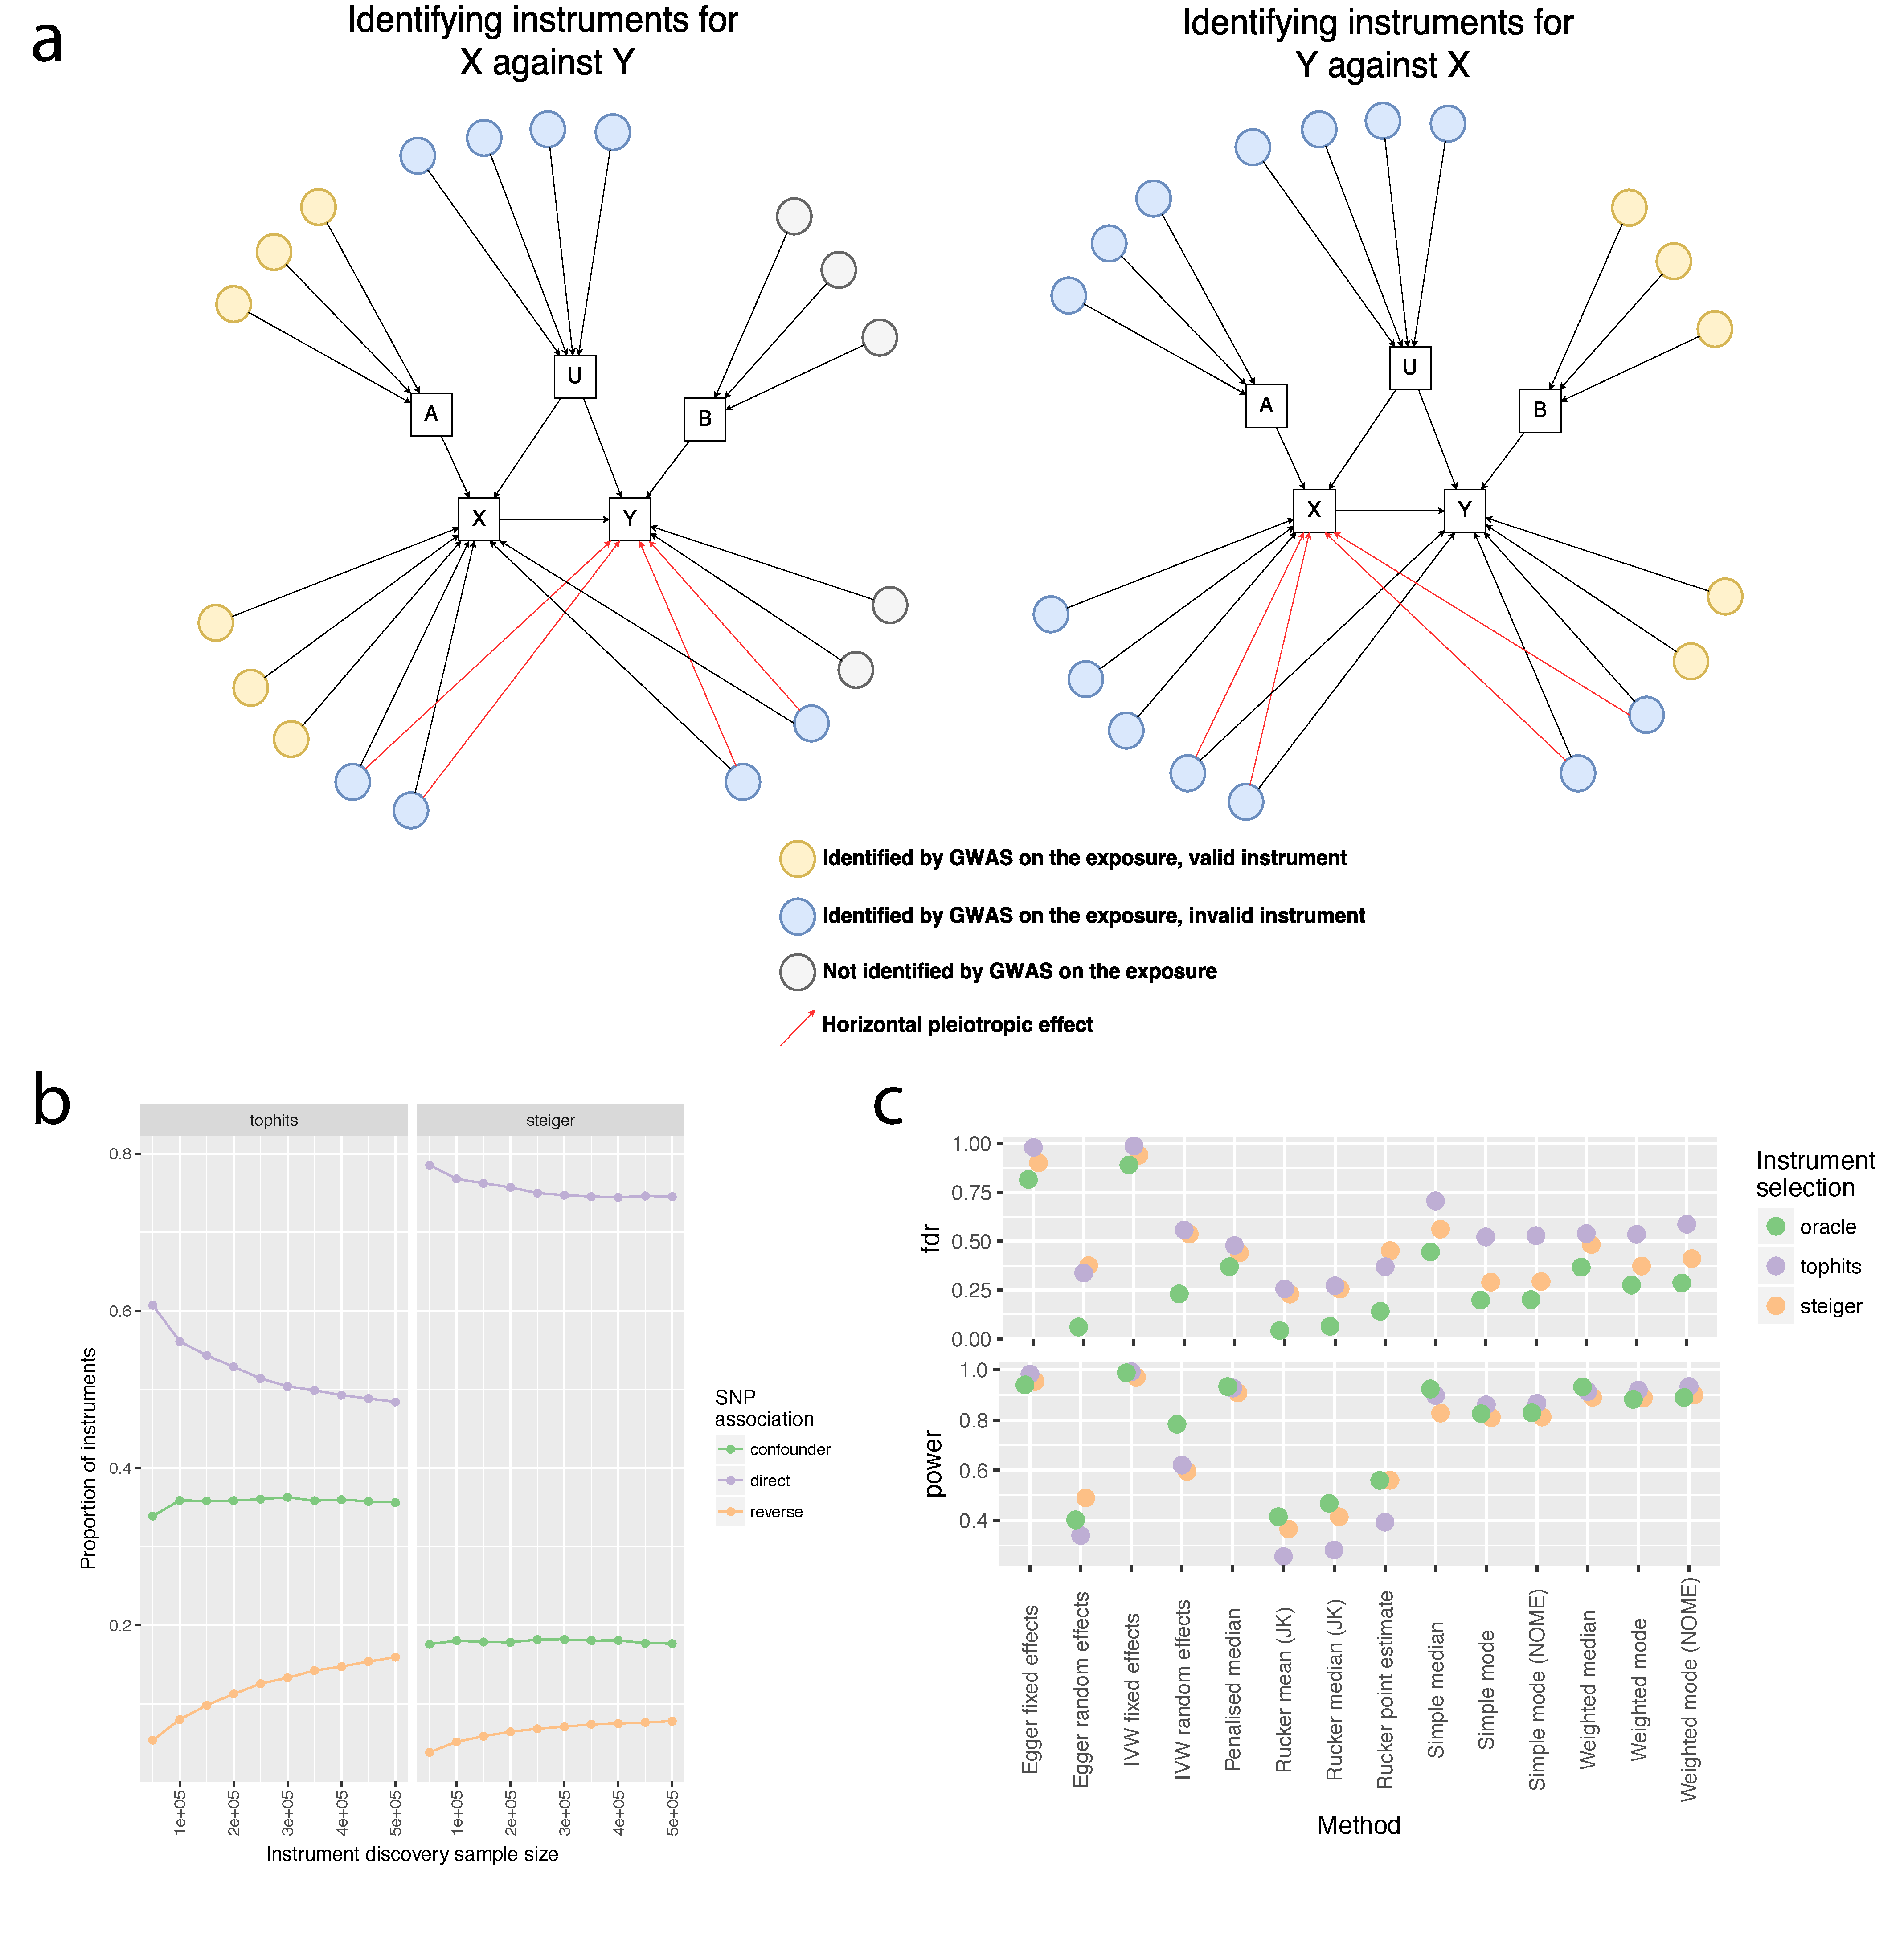
\includegraphics{images/fig1.pdf}

\newpage

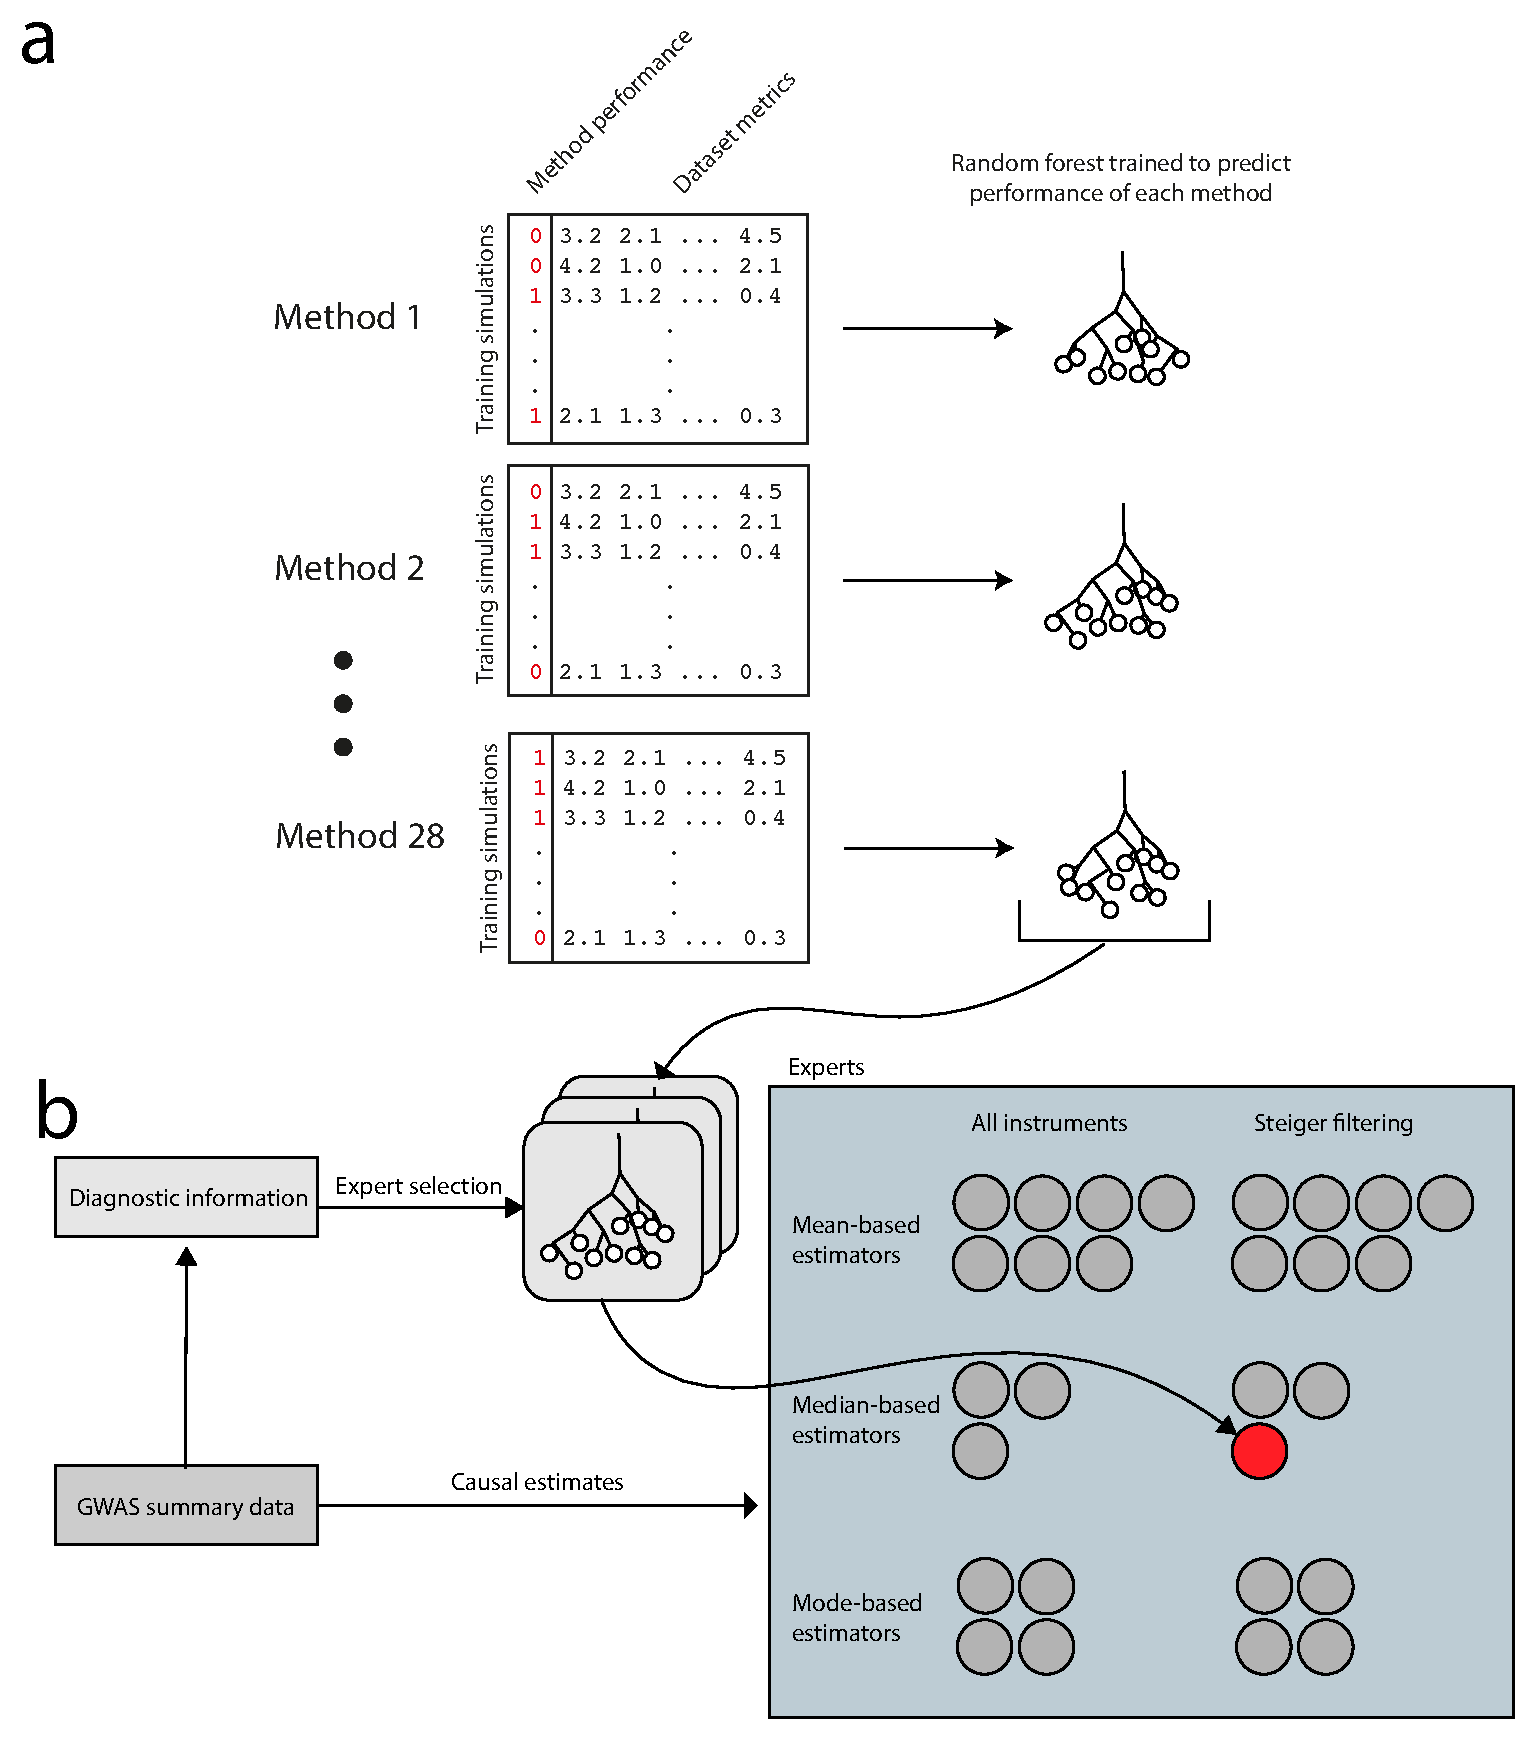
\includegraphics{images/fig2.pdf}

\subsection*{References}\label{references}
\addcontentsline{toc}{subsection}{References}

\hypertarget{refs}{}
\hypertarget{ref-DaveySmith2003}{}
1. Davey Smith G, Ebrahim S. 'Mendelian randomization': can genetic
epidemiology contribute to understanding environmental determinants of
disease? International Journal of Epidemiology {[}Internet{]}. 2003
Feb;32(1):1--22. Available from:
\url{http://www.ije.oxfordjournals.org/cgi/doi/10.1093/ije/dyg070}

\hypertarget{ref-DaveySmithHemani2014}{}
2. Davey Smith G, Hemani G. Mendelian randomization: genetic anchors for
causal inference in epidemiological studies. Human molecular genetics.
2014 Jul;23(R1):R89-----R98.


\end{document}
